% Fig. N1: New-configuration PSO optimization process
\begin{figure*}[t]
  \centering
  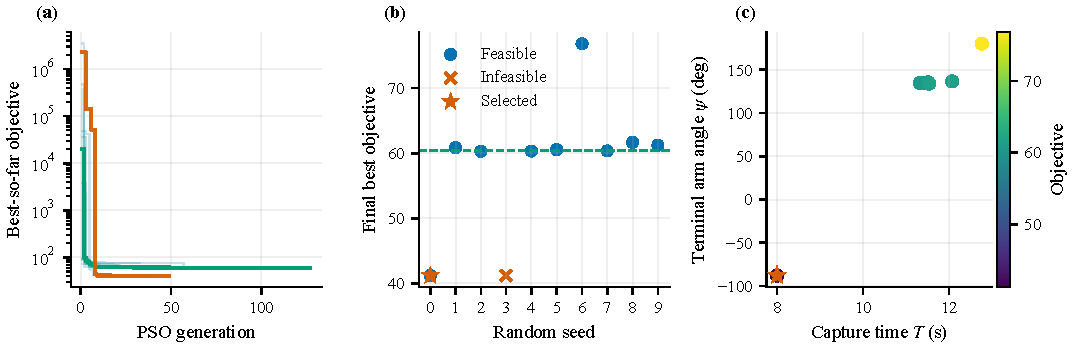
\includegraphics[width=0.98\textwidth]{../output/fpmfc/visualization/adaptive_cube_c095_014_095_face_aligned_v2_selected/fig_optimization_process.pdf}
  \caption{Particle-swarm optimization under the updated target position and face-to-face terminal-orientation constraint. The panels show best-so-far convergence over ten fixed seeds, final seed objectives with feasibility, and the distribution of capture time and terminal arm-shape angle.}
  \label{fig:new_target_optimization}
\end{figure*}

% Fig. N2: Selected 500 Hz pre-contact replay
\begin{figure*}[t]
  \centering
  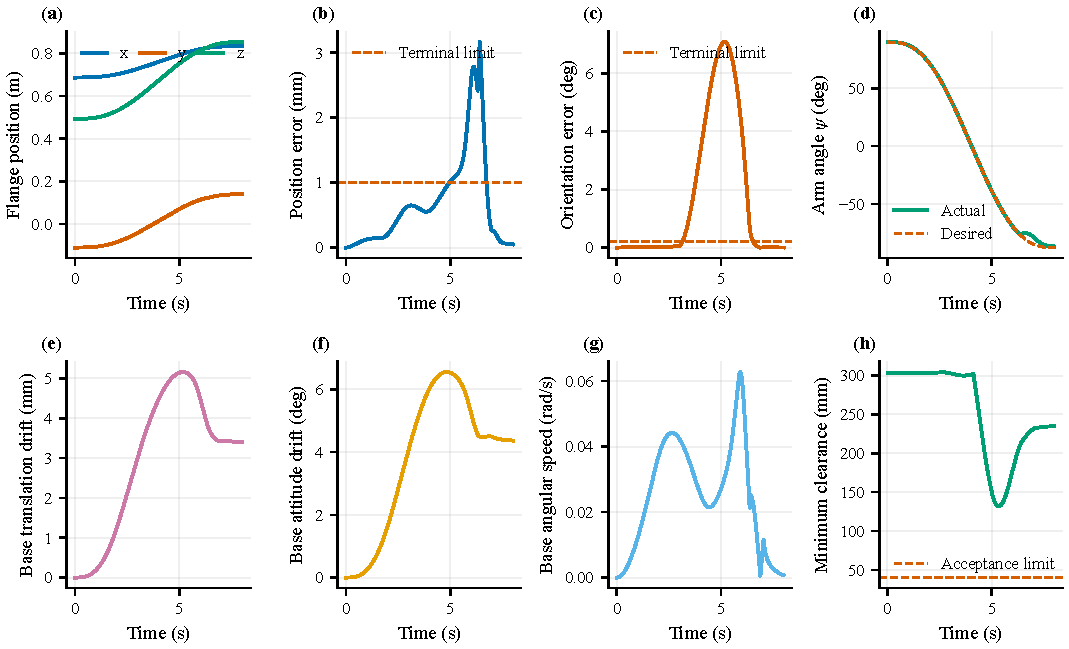
\includegraphics[width=0.98\textwidth]{../output/fpmfc/visualization/adaptive_cube_c095_014_095_face_aligned_v2_selected/fig_tracking_error_base_drift.pdf}
  \caption{Selected 500-Hz torque-level pre-contact replay for the updated geometry. End-effector tracking, transient position and orientation errors, arm-shape tracking, base translation and attitude drift, base angular speed, and minimum clearance are shown. Dashed position and orientation thresholds are terminal acceptance limits, not all-time tracking bounds.}
  \label{fig:new_target_dynamic_replay}
\end{figure*}
